\chapter{Lecture Exercises}

\section{11.09.24 - Exercise 1 - Replication, Transcription and Translation in prokaryotes}
For an automated version of answering this exercise, please see the file w2e1.py in the Python folder. This file will automatically replicate, transcribe and translate the given DNA sequence. Use the file as a template for future exercises if needed.

Figure \ref*{fig:Exercise1Seq} shows a DNA sequence which will used in Exercise 1 and its sub tasks. The given DNA sequence can be seen in figure \ref{fig:Exercise1Seq}

\begin{figure}[h]
    \centering  
    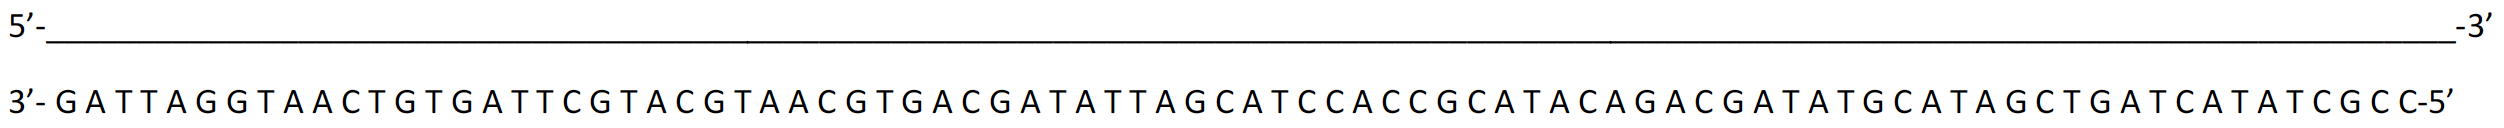
\includegraphics[width=1\textwidth]{Figures/Exercise1Seq.png}
    \caption{Sequence of DNA which is used in Exercise 1}
    \label{fig:Exercise1Seq}
\end{figure}
\subsection{Replication in prokaryotes}
Replicate the DNA sequence based on the anti-sense (template) strand written below using the following primer \textbf{5’- AUCCAUU -3’} (This RNA complementary to the DNA sequence and is the defined -35 region, which will be used in the transcription subsection).

\vspace{1em}
\begin{itemize}
    \item While replicating the DNA, identify the leading and lagging strands. Furthermore remember that G and C are the most stable base pairs, A and T are the least stable base pairs
    \item The DNA sequence is replicated from the 3’ to 5’ direction
    \item Use the primer as to define where to start from
\end{itemize} 

\vspace{1em}

5'- X X X \textbf{A T C C A} \textbf{\sethlcolor{Turquoise}\hl{T T G A C A}} C T A A G C A T G C A T T G C A C T G C \sethlcolor{green}\hl{\textbf{T A T A A T}} C G T A G G T G G C G T \textbf{\sethlcolor{Apricot}\hl{A T G}} T C T G C T A T A C G T A T C G A C T A G T A \textbf{\sethlcolor{Bittersweet}\hl{T A G}} C G G -3'      (This is the replicated)

\vspace{1em}

3’- \textit{G A T} \sethlcolor{yellow}\hl{\textbf{T A G G T A A}} C T G T G A T T C G T A C G T A A C G T G A C G A T A T T A G C A T C C A C C G C A T A C A G A C G A T A T G C A T A G C T G A T C A T A T C G C C-5’      (This is the given)

\vspace{1em}

So, to begin with, we will look at the given RNA primer, and convert it to a DNA primer.
5'-AUCCAUU-3' will be converted to 5'-ATCCATT-3' (since RNA has Uracil instead of Thymine). 


Afterwards we will look at the given DNA sequence and find the complementary strand to it. The complementary strand will be the anti-sense strand. 5'-ATCCATT-3' will be converted to 3'-TAGGTA-5' (since A pairs with T, T pairs with A, C pairs with G, and G pairs with C).


Now we will highlight the given sequence in \hl{yellow} and start translating the DNA sequence from the 3' to 5' direction. We will start from the primer and move towards the end of the sequence.

\vspace{1em}
This concludes this part of the exercise.

\subsection{Transcription in prokaryotes}
Identify the Pribnow (-10 region) and (-35) regions in the above DNA double-helix (sense strand). Transcribe DNA into a Messenger-RNA (mRNA).

\vspace{1em}
In this course the Pribnow box (-10 region) is defined as the region 5’-TATAAT-3’ and the -35 region is defined as 5’-TTGACA-3’. Wil will therefore 

We found the Pribnow box sequence and highlighted it in \sethlcolor{green}\hl{green}. The mRNA strand will be transcribed from the anti-sense strand, so we will use the antis sense strand to transcribe the mRNA until the -35 region which we highlighted in \sethlcolor{Turquoise}\hl{turquoise}.


We can now go to the right end (10-ish letters) of the pribnow box and start transcribing the mRNA. In this course, the start codon is defined as the first AUG codon after the Pribnow box. The mRNA strand will be transcribed from the 3' to 5' direction.

The start codon is highlighted in \sethlcolor{apricot}\hl{apricot} starting from the 13\textsuperscript{th} letter to the right. The stop codon is highlighted in \sethlcolor{Bittersweet}\hl{bittersweet}.


The Pribnow 10 region is \textbf{5’- ATCCATT -3’} and the -35 region is \textbf{5’- CGATAGG -3’}.

Now that we have identified both the start- and stop codon, we can start to transcribe the mRNA strand. The first codon will start from number 10 after the the Pribnow box. The mRNA strand will therefore be: 

\sethlcolor{CarnationPink}\hl{5'- GUA UGU CUG CUA UAC GUA UCG ACU AGU AUA GCG -3'}

\subsection{Translation in prokaryotes}
Translate the mRNA strand from transcription step into amino acids.

\vspace{1em}
The mRNA strand is written in the last subtask, and have already been translated into codons. It's now possible to translate the codons to amino acids.

H\textsubscript{2}N- Val - Cys - Leu - Leu - Tyr - Val - Ser - Thr - Ser - Iso - Ala -COOH

\section{11.09.24 - Exercise 2 - PCR and Restriction Enzymes}
A part of DNA fragment shown below is to be amplified using PCR and the primers F and R.  Subsequently the PCR product is cut with restriction enzyme HpyCH4V and the resultant products are run on a gel. The

\begin{figure}[h]
    \centering
    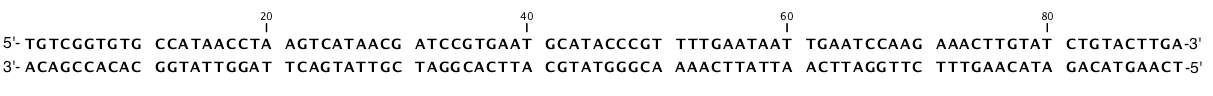
\includegraphics[width=1\textwidth]{Figures/Exc2DNA.png}
    \caption{Sequence of DNA which is used in Exercise 2}
    \label{fig:Exercise2Seq}
\end{figure}

The two given primers are:
\begin{itemize}
    \item Primer F: 5’- AACCT-3’
    \item Primer R: 5’-TGGAT-3’ (3'-TAGGT-5')
\end{itemize}

\subsection{What is the size (in base pairs) of the PCR-product?}
The Primer F starts from the 3' end of the DNA sequence, and the Primer R starts from the 5' end of the DNA sequence. The PCR product will therefore be the DNA sequence between the two primers.

Primer F has to fit to the upper strand, and Primer R has to fit on the lower strand. The primners sequence are therefore:
\begin{itemize}
    \item Primer F: 5'-AACCT-3' 
    \item Primer R: 5'-TGGAT-3' -> 3'-TAGGT-5'
\end{itemize}

Primer F starts from the 15\textsuperscript{th} to the right and ends at the 19\textsuperscript{th} base pair. Primer R starts from the 64\textsuperscript{th} from the right and ends at the 68\textsuperscript{th} base pair. The PCR product will therefore be the DNA sequence between the 19\textsuperscript{th} and 64\textsuperscript{th} base pair.

\underline{The size of the PCR-product is therefore 68-14 = 54 base pairs.}

\subsection{How many copies of DNA do you have after 4 PCR cycles if you start with 3 copies of the DNA- fragment to be copied (considering ideal conditions)?}
After each PCR cycle, the amount of DNA doubles. After 4 PCR cycles, the amount of DNA will be 2\textsuperscript{4} = 16 times the original amount of DNA.
Though, we are starting with 3 copies of the DNA fragment, so the amount of DNA after 4 PCR cycles will be $3 \cdot 2^4$ = 48 copies of the DNA fragment.

\subsection{What is the size of 2 fragments after cutting with HpyCH4V?}
The restriction enzyme HpyCH4V recognizes the sequence 3'-ACGT-5'. The DNA sequence is cut at the recognition site, and the two fragments will be the DNA sequence before the recognition site and the DNA sequence after the recognition site.

5'- TGTCGGTGTG CCATAACCTA AGTCATAACG ATCCGTGAAT GCATACCCGT TTTGAATAAT TGAATCCAAG AAACTTGTAT CTGTACTTGA-3'

3'- ACAGCCACAC GGTATTGGAT TCAGTATTGC TAGGCACTTA CGTATGGGCA AAACTTATTA ACTTAGGTTC TTTGAACATA GACATGAACT-5'
\vspace{1em}

HpyCH4V will therefore cut the DNA sequence at number 41, and the two fragments will be:

5'- AACCTA AGTCATAACG ATCCGTGAA\textbf{T GCA}TACCCGT TTTGAATAAT TGAATCCA-3'

3'- TTGGAT TCAGTATTGC TAGGCACTT\textbf{A CGT}ATGGGCA AAACTTATTA ACTTAGGT-5'

\vspace{1em}   
\underline{There will therefore be 27 base pairs in the first fragment and 27 base pairs in the second fragment.}

\subsection{Place the bands that you would observe after running your product on the an agarose gel (path 1 before cutting with enzyme, path 2 after cutting)}

When you run the PCR product on a gel electroforesis, you will see the DNA fragments separated based on their size. The smaller fragments will move faster through the gel than the larger fragments. This means that both the DNA fragment before and after cutting with the restriction enzyme will be visible on the gel since they doesn't have the same fragment size   .

Therefore you will see two bands on the gel, one at 54 base pairs (before cutting) and one at 27 base pairs (after cutting).
This can be seen in Figure \ref{fig:Exercise2Gel}.
\clearpage
\begin{figure}[t]
    \centering
    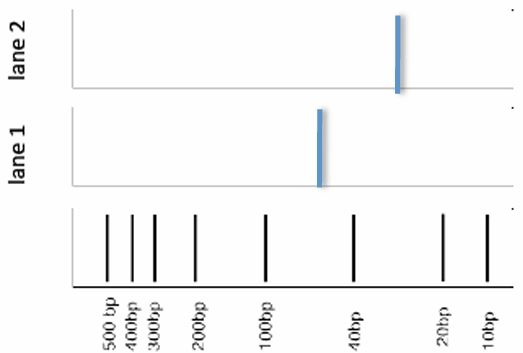
\includegraphics[angle=270, width=0.35\textwidth]{Figures/Exc2Gel.JPG}
    \caption{Gel electrophoresis of the DNA fragments and the PCR products' bands}
    \label{fig:Exercise2Gel}
\end{figure}

\section{11.09.24 - Exercise 3 - Primer3plus}
Based on the sequence below design primers that fulfill following conditions:

The following information is given:

\begin{highlight}
    \begin{itemize}
        \item size (22-24bp)
        \item Tm (55-57)
        \item GC\% (35-70)
        \item amplicon size (300-400bp)
    \end{itemize}
\end{highlight}

The following sequence is given:

\begin{verbatim}
    TTGCAAGCCCTGATTTAAGCATTACACCAGCATCATCAAAGTAATACGCATTTCCATTTTGATCAGTTAT
    ATATTGGTCAAAAACTTGATGACCTTTCTTATCGAAATAAACAATTGTACCATCTTCGTTTTGTAAGAAG
    CTCTTGACCAGTTCGATACCATTAGGTAAGAAGAAGTAGGTATGGTTATTAATCTTTTGCAAACCTGTTA
    CTAAATGACCTGTTTTATCAAAATAGTAATAGTTATTATCATCATCTTGAATAAATGCATTTTGGGCACG
    ATAACCACTTAATGTATAATAGATGATTCCTTTATCATCGTGTGTAAAGCCAGTTTCTGACAGATCATTA
    GTTAACTGTTTTGGTAAGTAGTCACCATCCTCAGTGTTCGAAACGACCTTAAAGTACTTATCAGAACCCA
    TATCTTTCAATACGTATCCAGCACCTTTACCTTGGATGTTAGAGCCATTGAAGTACTTAGCCGCCCACTC
    AGTAATCTTTACACTGCCATCAATTGGAACGCCAGTTGAGATTTGATTCACTTTAAATAGGGATGGATAG
    AGTGCCTGTAACTCTTCTAAGAAGGCACCACCATACATCTCTTGATATTGACCACCCCCACGACTTTGTA
    CAACATATAAGGCATTGTCAATATCAGAATCTGTATCGTCATCTCCAAATGAATTTGTTCTTGTGACAGT
    AGCTAATTCTTGCTCTGGCAAATTATAAATTTGGTCCGGCACCCAATCGGCAATGGCTTGAATACCGCTA
    GCATGTAAGGCTTTAATAGCATCGCGCAACTGATCAGCAGTTCCATATTTTGTCGGTGTGCCATAACCTA
    AGTCATAACGATCCGTGAATGCATACCCGTTTTGAATAATTGAATCCAAGAAACTTGTATCTGTACTTGA
    ACGATATTGTGGTGCCAATTGGAAGCTTGTCACACCCCATTGCTTAAATTGGTCCGCATTCTGAGCGATG
    ACTACGTTTGTATATTCACTGCTGTCTGTAGCAAATGCTTGGAAGTTTGAGAAACCTTCGTAGATGACTT
    GAGAATCAAGAGCAGCGTTTGAATGGAACACTTTATCACTCGTGTTTGTTGTTGTATCAGAGGCCGTTCG
    TGCATCTTGATCTTGTTGCGCACCTACCGGAACCCAAACTGCCAAGTAACCAGAAACTTGTGGATTTTGT
    ACACCATAAATTGATTCATTCGTAAAAATCAAATCGCCGTTAGCATCTGTGTACGCCACAGGTGCATTTT
    CATCAGTATCATAATAAGCTAATCCATCTGCAGTTGTTGATAACAAAGCACGATAAGCTTGGTTCTTATG
    AGCTGCCCCCATATGCAATGTGACAGTATGCCCATCCTCTAATTGTAGCTCCGCGTTATTGCTGACGATG
    ACTCCAATACCTTCAGTACGCGTCTCAGATGTTCCAGTGTCAGAAGCCGTCATGGCATCTTTACCATAGC
    GAACACTTGTTAACACGTCATTACTATCAACGGACATCGATTGGCCACCAGCAACATATTGGACTCTAGC
    CTTCAGCAAAGTGTTAATCGCATCATAGTATGGTGACTTTGTTGCCATATATTGACCATCATCTGTATAT
    AAATCGCCATAATAGACACGAGGAACAGTATCCTTGTTGGTTAGCAACATCGCATAAGCACTAGCCATAT
    TATATTGTGTGTACTTTTTGTCTGCTAATTTTTCATCTTCATTGTATACTTTGAAAGCAGCTGCCAATTG
\end{verbatim}


\vspace{1em}
Use Primer3Plus (http://www.bioinformatics.nl/cgi-bin/primer3plus/primer3plus.cgi/)

\vspace{1em}
While setting the conditions, it's important to remember that the amplicon size is the size of the DNA fragment that will be amplified by the primers.This is named "Product range size" on the web-side under general settings.

\vspace{1em}
Write answers in the table bellow:
\begin{table}[h]
    \centering
    \caption{The given table which should be filled out with the information from the Primer3Plus web-side}
    \label{tab:Exercise3PrimerTable}
    \begin{tabular}{c|c|c|c|c}
        \textbf{Primer} & \textbf{Sequence (5'-3')} & \textbf{Primer size (bp)} & \textbf{Tm (°C)} & \textbf{GC content\%} \\
        \hline
        Forward & TCAGTAATCTTTACACTGCCATC & 23 & 56.1 & 39.1 \\
        Reverse & TTATGACTTAGGTTATGGCACAC & 23 & 56.1 & 39.1 \\
    \end{tabular}
\end{table}

The second part of this exercise was to use this information to deduct which bacteria this sequence belongs to. The sequence is from the bacteria \textit{Leuconostoc mesenteroides}.

\section{11.09.24 - Exercise 4 - Primers check and restriction enzymes}
The following information is given:
\begin{itemize}
    \item Primer F: 5’- GGAACCCAAACTGCCAAGT-3’
    \item Primer R: 5’-CCTCGTGTCTATTATGGCGATT-3’
\end{itemize}

Using \textbf{“In silico PCR amplification”} (http://insilico.ehu.es/PCR/) answer following questions:

\subsection{What \textit{Leuconostoc} strain will the primers align to?}
We start by going to the web-side. Then we choose \textit{Leuconostoc} and press "Next step". Afterwards we paste the primer sequences into the "Forward primer" and "Reverse primer" fields. We then choose "APPLY TO ALL Leuconostoc" and press "Amplify".

Then we can see 2 bands where the primers has traveled at 485 and 485 base pairs. The primers will therefore align to the 2 \textit{Leuconostoc mesenteroides} strains.

\subsection{What would be the PCR product size (bp) if we use those primers against that species?}
Based on the bands that was produced the PCR product size will be 485 base pairs.

\vspace{3em}
For the next subsections, the following information is given:

Using NEBcutter V2.O  http://tools.neb.com/NEBcutter2/ retrieve the amplicon from “In silico PCR amplification” and answer following questions:

\subsection{What will be the size of DNA products after digesting the amplicon with Hind III restriction enzyme?}
To use the web-side you need to copy the DNA sequence from the "In silico PCR amplification" web-side and paste it into the "Enter DNA sequence" field and press sumbit. Then you look at the sumary and find the restriction enzyme HendIII and hold the mouse over it to see where it cuts. 

\vspace{1em}
For the two \textit{Leuconostoc} strains the HINDIII cuts at:
\begin{itemize}
    \item Cuts at bp 167 (Leuconostoc mesenteroides subsp. mesenteroides ATCC 8293)
    \item Cuts at bp 167 (Leuconostoc mesenteroides subsp. mesenteroides J18)
\end{itemize}

\vspace{1em}
This means that the DNA products will be 167- and 318 base pairs long after digesting the amplicon with HindIII restriction enzyme. This makes sense since the total sequence, for both, is 485 base pairs long. Thus 167+318 = 485 base pairs.

\subsection{What are the reaction conditions requires for ApeKI?}
To answer this, the following table has to be filled out. The information can be found on the NEBcutter web-side by pressing "Enzyme list" and then "ApeKI". Then in the bottom right corner of the first table, there is a button called "NEV Restriction Enzyme - Activity/Performance Chart". Then find the enzyme ApeKI and press on the buffer, there all the needed information is found. 

\begin{table}[h]
    \centering
    \caption{The given table which should be filled out with the information from the NEBcutter web-side}
    \label{tab:Exc4ApeKI}
    \begin{tabular}{c|c}
        \textbf{Buffer} & \textbf{NEBuffer\textsuperscript{TM} r3.1} \\
        \hline
        Salt & 100 mM NaCl \\
        Main & 50 mM Tris-HCl \\
        pH & 7.9 at 25\textdegree C  \\
        Mg & 10 mM MgCl\textsubscript{2} \\
        rAlbumin & 100 \textmu g/ml Recombinant Albumin\\
        Reaction temp. (\textdegree C) & 75\textdegree C (Obtained from the solutions)\\
    \end{tabular}
\end{table}

\subsection{What is the digestion pattern of AciI?}
The AciI enzyme cuts at the following base pairs:

Primer F 5'-...AA\textsuperscript{$\downarrow$}CGTT...-3'

Primer R 3'-...TTGC\textsubscript{$\uparrow$}AA...-5'

This information can be found on the page before you press "NEV Restriction Enzyme - Activity/Performance Chart".

\subsection{Using ENDMEMO}

For this exercise we need to use this web-side (http://www.endmemo.com/bio/egel.php)
In the graph on the right place bands you would  receive after digesting the amplicon with HindIII, ApeKI and AciI in one reaction. 

Here we simply need to insert a sequence and choose the right restriction enzymes. The bands will then be shown on the gel.

\begin{itemize}
    \item HindIII cuts at 167 bp; bands will be at 167- and 318 bp
    \subitem Blue color
    \item ApeKI cuts at 184 bp; bands will be at 184- and 301 bp
    \subitem Green color
    \item AciI cuts at 233 bp; bands will be at 233- and 252 bp
    \subitem Red color
\end{itemize}

\begin{figure}{h}
    \centering
    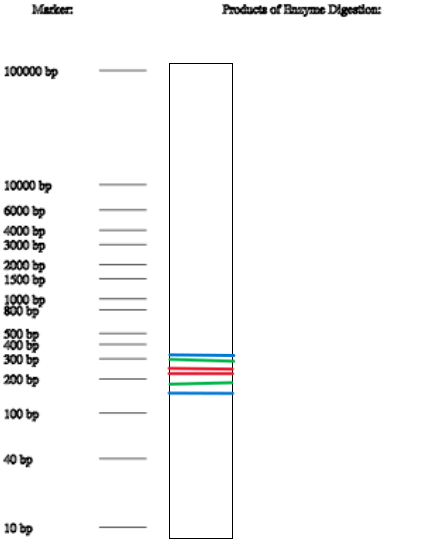
\includegraphics[width=0.35\textwidth]{Figures/Exc4sub6.png}
    \caption{Gel electrophoresis of the DNA fragments and the PCR products' bands}
    \label{fig:Exc4sub6}
\end{figure}
